% Options for packages loaded elsewhere
% Options for packages loaded elsewhere
\PassOptionsToPackage{unicode}{hyperref}
\PassOptionsToPackage{hyphens}{url}
%
\documentclass[
  ignorenonframetext,
]{beamer}
\newif\ifbibliography
\usepackage{pgfpages}
\setbeamertemplate{caption}[numbered]
\setbeamertemplate{caption label separator}{: }
\setbeamercolor{caption name}{fg=normal text.fg}
\beamertemplatenavigationsymbolsempty
% remove section numbering
\setbeamertemplate{part page}{
  \centering
  \begin{beamercolorbox}[sep=16pt,center]{part title}
    \usebeamerfont{part title}\insertpart\par
  \end{beamercolorbox}
}
\setbeamertemplate{section page}{
  \centering
  \begin{beamercolorbox}[sep=12pt,center]{section title}
    \usebeamerfont{section title}\insertsection\par
  \end{beamercolorbox}
}
\setbeamertemplate{subsection page}{
  \centering
  \begin{beamercolorbox}[sep=8pt,center]{subsection title}
    \usebeamerfont{subsection title}\insertsubsection\par
  \end{beamercolorbox}
}
% Prevent slide breaks in the middle of a paragraph
\widowpenalties 1 10000
\raggedbottom
\AtBeginPart{
  \frame{\partpage}
}
\AtBeginSection{
  \ifbibliography
  \else
    \frame{\sectionpage}
  \fi
}
\AtBeginSubsection{
  \frame{\subsectionpage}
}
\usepackage{iftex}
\ifPDFTeX
  \usepackage[T1]{fontenc}
  \usepackage[utf8]{inputenc}
  \usepackage{textcomp} % provide euro and other symbols
\else % if luatex or xetex
  \usepackage{unicode-math} % this also loads fontspec
  \defaultfontfeatures{Scale=MatchLowercase}
  \defaultfontfeatures[\rmfamily]{Ligatures=TeX,Scale=1}
\fi
\usepackage{lmodern}

\usetheme[]{metropolis}
\ifPDFTeX\else
  % xetex/luatex font selection
\fi
% Use upquote if available, for straight quotes in verbatim environments
\IfFileExists{upquote.sty}{\usepackage{upquote}}{}
\IfFileExists{microtype.sty}{% use microtype if available
  \usepackage[]{microtype}
  \UseMicrotypeSet[protrusion]{basicmath} % disable protrusion for tt fonts
}{}
\makeatletter
\@ifundefined{KOMAClassName}{% if non-KOMA class
  \IfFileExists{parskip.sty}{%
    \usepackage{parskip}
  }{% else
    \setlength{\parindent}{0pt}
    \setlength{\parskip}{6pt plus 2pt minus 1pt}}
}{% if KOMA class
  \KOMAoptions{parskip=half}}
\makeatother


\usepackage{longtable,booktabs,array}
\usepackage{calc} % for calculating minipage widths
\usepackage{caption}
% Make caption package work with longtable
\makeatletter
\def\fnum@table{\tablename~\thetable}
\makeatother
\usepackage{graphicx}
\makeatletter
\newsavebox\pandoc@box
\newcommand*\pandocbounded[1]{% scales image to fit in text height/width
  \sbox\pandoc@box{#1}%
  \Gscale@div\@tempa{\textheight}{\dimexpr\ht\pandoc@box+\dp\pandoc@box\relax}%
  \Gscale@div\@tempb{\linewidth}{\wd\pandoc@box}%
  \ifdim\@tempb\p@<\@tempa\p@\let\@tempa\@tempb\fi% select the smaller of both
  \ifdim\@tempa\p@<\p@\scalebox{\@tempa}{\usebox\pandoc@box}%
  \else\usebox{\pandoc@box}%
  \fi%
}
% Set default figure placement to htbp
\def\fps@figure{htbp}
\makeatother





\setlength{\emergencystretch}{3em} % prevent overfull lines

\providecommand{\tightlist}{%
  \setlength{\itemsep}{0pt}\setlength{\parskip}{0pt}}



 


\setbeamerfont{title}{size=\large}
\usepackage{hyperref}
\setbeamertemplate{footline}[frame number]
\usepackage{tikz}
\usetikzlibrary{arrows.meta, positioning, shapes.geometric, fit, backgrounds, calc}
\usepackage{booktabs}
\usepackage{xcolor}
\usepackage{array}
\usepackage{colortbl}
\definecolor{mblue}{RGB}{35,55,100}
\definecolor{mred}{RGB}{160,30,30}
\definecolor{mgreen}{RGB}{30,100,60}
\makeatletter
\@ifpackageloaded{caption}{}{\usepackage{caption}}
\AtBeginDocument{%
\ifdefined\contentsname
  \renewcommand*\contentsname{Table of contents}
\else
  \newcommand\contentsname{Table of contents}
\fi
\ifdefined\listfigurename
  \renewcommand*\listfigurename{List of Figures}
\else
  \newcommand\listfigurename{List of Figures}
\fi
\ifdefined\listtablename
  \renewcommand*\listtablename{List of Tables}
\else
  \newcommand\listtablename{List of Tables}
\fi
\ifdefined\figurename
  \renewcommand*\figurename{Figure}
\else
  \newcommand\figurename{Figure}
\fi
\ifdefined\tablename
  \renewcommand*\tablename{Table}
\else
  \newcommand\tablename{Table}
\fi
}
\@ifpackageloaded{float}{}{\usepackage{float}}
\floatstyle{ruled}
\@ifundefined{c@chapter}{\newfloat{codelisting}{h}{lop}}{\newfloat{codelisting}{h}{lop}[chapter]}
\floatname{codelisting}{Listing}
\newcommand*\listoflistings{\listof{codelisting}{List of Listings}}
\makeatother
\makeatletter
\makeatother
\makeatletter
\@ifpackageloaded{caption}{}{\usepackage{caption}}
\@ifpackageloaded{subcaption}{}{\usepackage{subcaption}}
\makeatother

\usepackage{bookmark}
\IfFileExists{xurl.sty}{\usepackage{xurl}}{} % add URL line breaks if available
\urlstyle{same}
\hypersetup{
  pdfauthor={Giorgio Arcara},
  hidelinks,
  pdfcreator={LaTeX via pandoc}}


\author{Giorgio Arcara}
\date{}

\begin{document}


\begin{frame}
\title{Metodologia della Ricerca Clinica\\
\vspace{0.5em}
{\normalsize \textbf{APPENDICE --- Regressione Lineare e Logistica}}}
\author{Giorgio Arcara,\\ Università di Padova \\ IRCCS San Camillo, Venezia}
\titlegraphic{
\vspace*{7cm}
\includegraphics[scale=0.15]{Figures/LogoSanCamilloIRCCS_Unipd_alpha.png}
\hfill \includegraphics[scale=0.15]{Figures/CC_license_3_0.png}
}
\maketitle
\end{frame}

\section{Introduzione ai Modelli di
Regressione}\label{introduzione-ai-modelli-di-regressione}

\begin{frame}{Perché la Regressione?}
\phantomsection\label{perchuxe9-la-regressione}
\small

La regressione è lo strumento statistico più usato nella ricerca clinica
per:

\begin{itemize}\footnotesize
\item Descrivere la relazione tra una variabile dipendente e uno o più predittori
\item Controllare statisticamente per variabili confondenti
\item Predire un outcome a partire da un insieme di variabili
\item Quantificare la dimensione dell'effetto di un predittore \emph{tenendo costanti gli altri}
\end{itemize}

\vspace{0.4em}

\begin{center}
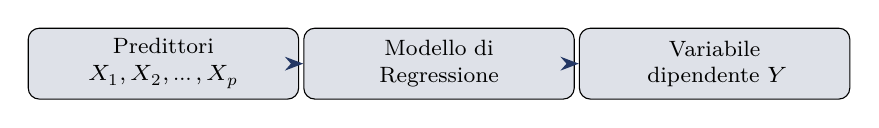
\begin{tikzpicture}[
  box/.style={draw,rounded corners,fill=mblue!15,text width=3.2cm,
              align=center,font=\footnotesize,minimum height=0.9cm},
  arr/.style={-{Stealth},mblue,thick}
]
\node[box] (x1) at (-3.5,0) {Predittori\\$X_1, X_2, \ldots, X_p$};
\node[box] (mod) at (0,0)   {Modello di\\Regressione};
\node[box] (y)  at (3.5,0)  {Variabile\\dipendente $Y$};
\draw[arr] (x1)--(mod); \draw[arr] (mod)--(y);
\end{tikzpicture}
\end{center}

\vspace{0.3em}

\small Due domande distinte: \textbf{(1) spiegazione} --- quali
predittori sono associati a \(Y\) e di quanto? \textbf{(2) predizione}
--- quanto accuratamente posso stimare \(Y\) per un nuovo soggetto?
\end{frame}

\begin{frame}{Regressione Lineare vs Logistica: Quando Usarle}
\phantomsection\label{regressione-lineare-vs-logistica-quando-usarle}
\begin{center}
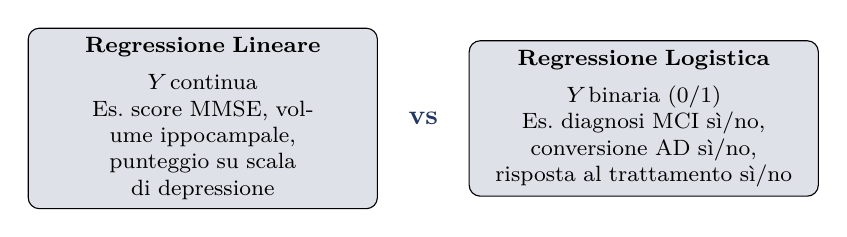
\begin{tikzpicture}[
  box/.style={draw,rounded corners,fill=mblue!15,text width=4.2cm,
              align=center,font=\footnotesize,minimum height=1.3cm},
]
\node[box] (lin) at (-2.8,0) {
  \textbf{Regressione Lineare}\\[4pt]
  \footnotesize $Y$ continua\\
  Es.\ score MMSE, volume ippocampale,\\
  punteggio su scala di depressione
};
\node[box] (log) at (2.8,0) {
  \textbf{Regressione Logistica}\\[4pt]
  \footnotesize $Y$ binaria (0/1)\\
  Es.\ diagnosi MCI sì/no,\\
  conversione AD sì/no,\\
  risposta al trattamento sì/no
};
\node[font=\normalsize\bfseries,mblue] at (0,0) {vs};
\end{tikzpicture}
\end{center}
\vspace{0.4em}
\small \textbf{Nota}: esistono estensioni per outcome ordinali (regressione ordinale), conteggi (Poisson), tempi all'evento (Cox) --- ma lineare e logistica coprono la maggioranza delle situazioni in neuropsicologia.
\end{frame}

\section{Regressione Lineare}\label{regressione-lineare}

\begin{frame}{Il Modello}
\phantomsection\label{il-modello}
\small

\[Y_i = \beta_0 + \beta_1 X_{1i} + \beta_2 X_{2i} + \ldots + \beta_p X_{pi} + \varepsilon_i\]

dove \(\varepsilon_i \sim \mathcal{N}(0, \sigma^2)\) (errori i.i.d.,
distribuzione normale).

\vspace{0.4em}

\textbf{Interpretazione dei coefficienti} \(\beta_j\):

\begin{itemize}\footnotesize
\item $\beta_0$: valore atteso di $Y$ quando tutti i predittori = 0 (intercetta)
\item $\beta_j$: variazione attesa di $Y$ per un incremento unitario di $X_j$,\\ \textbf{tenendo costanti tutti gli altri predittori}
\end{itemize}

\vspace{0.4em}

\textbf{Stima}: minimi quadrati ordinari (OLS) --- minimizza
\(\sum_i (Y_i - \hat{Y}_i)^2\).

\vspace{0.4em}

\textbf{Misure di fit}:

\begin{itemize}\footnotesize
\item $R^2$: proporzione di varianza di $Y$ spiegata dal modello
\item $R^2$ aggiustato: penalizza per il numero di predittori
\item RMSE (Root Mean Squared Error): errore medio in unità di $Y$
\end{itemize}
\end{frame}

\begin{frame}{Output di una Regressione Lineare (come appare in un
articolo)}
\phantomsection\label{output-di-una-regressione-lineare-come-appare-in-un-articolo}
\vspace{-0.2em}
\begin{center}
\small
\textbf{Tabella 1.} Predittori dello score MMSE in pazienti con MCI ($N = 120$)
\vspace{0.4em}

\begin{tabular}{lrrrr}
\toprule
\textbf{Predittore} & $\boldsymbol{\hat{\beta}}$ & \textbf{SE} & \textbf{95\% CI} & $\boldsymbol{p}$ \\
\midrule
Intercetta           & 34.21 & 2.18 & [29.90, 38.52] & $<.001$ \\
\rowcolor{mblue!8}
Età (anni)           & $-0.18$ & 0.04 & [$-0.26$, $-0.10$] & $<.001$ \\
Scolarità (anni)     & $+0.31$ & 0.07 & [$+0.17$, $+0.45$] & $<.001$ \\
\rowcolor{mblue!8}
Depressione (GDS)    & $-0.22$ & 0.09 & [$-0.40$, $-0.04$] & $.018$  \\
Sesso (F vs M)       & $-0.41$ & 0.48 & [$-1.36$, $+0.54$] & $.393$  \\
\midrule
\multicolumn{5}{l}{\footnotesize $R^2 = .38$; \; $R^2_{\text{adj}} = .36$; \; $F(4, 115) = 17.6$, $p < .001$} \\
\bottomrule
\end{tabular}
\end{center}
\vspace{0.2em}
\footnotesize
\textbf{Lettura}: Ogni anno in più di età è associato a un punteggio MMSE inferiore di 0.18 punti ($p < .001$), tenendo costanti scolarità, depressione e sesso. Il sesso non è un predittore significativo in questo modello ($p = .393$).
\end{frame}

\begin{frame}{Come Leggere i Coefficienti (Regressione Lineare)}
\phantomsection\label{come-leggere-i-coefficienti-regressione-lineare}
\small

\textbf{Predittore continuo} (es.~scolarità):

\(\hat{\beta} = +0.31\) significa: per ogni anno aggiuntivo di
scolarità, il punteggio MMSE aumenta di 0.31 punti \emph{in media},
tenendo costanti gli altri predittori.

\vspace{0.4em}

\textbf{Predittore categoriale binario} (es.~sesso F vs M):

\(\hat{\beta} = -0.41\) significa: le donne hanno un punteggio MMSE
mediamente inferiore di 0.41 punti rispetto agli uomini, tenendo
costanti gli altri predittori. (Non significativo: \(p = .393\).)

\vspace{0.4em}

\textbf{Intervallo di confidenza al 95\%}: l'intervallo che, se
ripetessimo lo studio infinite volte, conterrebbe il vero parametro nel
95\% dei casi. Se l'IC \textbf{non include lo zero} \(\Rightarrow\)
significativo a \(\alpha = 0.05\).

\vspace{0.4em}

\textbf{Attenzione alle unità}: \(\hat{\beta}\) dipende dalle unità di
misura del predittore. Per confrontare l'importanza relativa di
predittori con scale diverse, usare i
\textbf{coefficienti standardizzati} (\(\beta^*\)).
\end{frame}

\section{Regressione Logistica}\label{regressione-logistica}

\begin{frame}{Il Problema con una Variabile Dipendente Binaria}
\phantomsection\label{il-problema-con-una-variabile-dipendente-binaria}
\end{frame}

\begin{frame}{Il Modello Logistico}
\phantomsection\label{il-modello-logistico}
\small

\[\log\left(\frac{p_i}{1-p_i}\right) = \beta_0 + \beta_1 X_{1i} + \ldots + \beta_p X_{pi}\]

Il termine a sinistra è il \textbf{logit} (log-odds): il logaritmo del
rapporto tra la probabilità dell'evento e quella del non-evento.

\vspace{0.3em}

Invertendo:
\[p_i = \frac{1}{1 + e^{-(\beta_0 + \beta_1 X_{1i} + \ldots)}}\]

\vspace{0.3em}

\textbf{Stima}: massima verosimiglianza (ML), non minimi quadrati.

\vspace{0.3em}

\textbf{Misure di fit}:

\begin{itemize}\footnotesize
\item Log-likelihood, AIC, BIC (più bassi = meglio)
\item $R^2$ di Nagelkerke, McFadden (pseudo-$R^2$, non identici al $R^2$ lineare)
\item Hosmer-Lemeshow test (calibrazione)
\item AUC-ROC (discriminazione)
\end{itemize}
\end{frame}

\begin{frame}{L'Odds Ratio: Intuizione}
\phantomsection\label{lodds-ratio-intuizione}
\small

Il coefficiente \(\hat{\beta}_j\) della logistica non si interpreta
direttamente come in quella lineare. Si usa l'\textbf{Odds Ratio} (OR):

\[OR_j = e^{\hat{\beta}_j}\]

\vspace{0.3em}

\textbf{Cos'è l'odds?}

\[\text{odds} = \frac{p}{1-p}\]

Se la probabilità di conversione ad AD è 0.25, l'odds è
\(0.25/0.75 = 0.33\) (1 conversione ogni 3 non-conversioni).

\vspace{0.4em}

\textbf{Cos'è l'Odds Ratio?}

È il \emph{rapporto} tra gli odds in due condizioni: trattato vs non
trattato, o per un incremento unitario di \(X\).

\[OR = \frac{\text{odds}(\text{esposto})}{\text{odds}(\text{non esposto})}\]
\end{frame}

\begin{frame}{L'Odds Ratio: Interpretazione Pratica}
\phantomsection\label{lodds-ratio-interpretazione-pratica}
\begin{center}
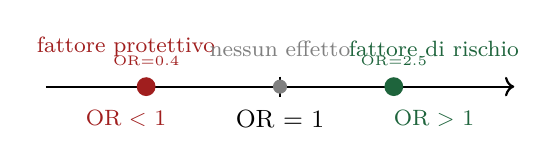
\begin{tikzpicture}[scale=0.85,
  arr/.style={-{Stealth},mblue,thick}
]
  \draw[thick,->] (0,0) -- (7,0);
  \draw[thick] (3.5,0.15)--(3.5,-0.15);
  \node[below,font=\small] at (3.5,-0.2) {OR = 1};
  \node[below,font=\footnotesize,mred] at (1.2,-0.2) {OR $<$ 1};
  \node[below,font=\footnotesize,mgreen] at (5.8,-0.2) {OR $>$ 1};
  \node[above,font=\footnotesize,mred] at (1.2,0.3) {fattore protettivo};
  \node[above,font=\footnotesize,gray] at (3.5,0.3) {nessun effetto};
  \node[above,font=\footnotesize,mgreen] at (5.8,0.3) {fattore di rischio};

  % Example OR markers
  \fill[mred]   (1.5,0) circle (4pt) node[above,font=\tiny,yshift=4pt]{OR=0.4};
  \fill[gray]   (3.5,0) circle (3pt);
  \fill[mgreen] (5.2,0) circle (4pt) node[above,font=\tiny,yshift=4pt]{OR=2.5};
\end{tikzpicture}
\end{center}
\vspace{0.2em}

\begin{longtable}[]{@{}
  >{\raggedright\arraybackslash}p{(\linewidth - 2\tabcolsep) * \real{0.5000}}
  >{\raggedright\arraybackslash}p{(\linewidth - 2\tabcolsep) * \real{0.5000}}@{}}
\toprule\noalign{}
\begin{minipage}[b]{\linewidth}\raggedright
OR
\end{minipage} & \begin{minipage}[b]{\linewidth}\raggedright
Interpretazione
\end{minipage} \\
\midrule\noalign{}
\endhead
\footnotesize \(OR = 1\) & \footnotesize Nessuna associazione \\
\footnotesize \(OR = 2.5\) & \footnotesize Gli esposti hanno odds di
evento 2.5 volte quelle dei non esposti \\
\footnotesize \(OR = 0.4\) & \footnotesize Gli esposti hanno odds di
evento il 60\% \emph{inferiori} rispetto ai non esposti \\
\bottomrule\noalign{}
\end{longtable}

\vspace{0.2em}

\footnotesize \textbf{Attenzione}: OR \(\neq\) Rischio Relativo (RR).
L'OR sovrastima il RR quando la prevalenza dell'outcome è alta
(\(>10\%\)). Per prevalenze basse, OR \(\approx\) RR.
\end{frame}

\begin{frame}{Odds Ratio: Esempio Numerico}
\phantomsection\label{odds-ratio-esempio-numerico}
\small

Studio su 200 pazienti MCI: 50 convertono ad AD entro 2 anni.

\vspace{0.4em}

\begin{center}
\begin{tabular}{lcc>{\bfseries}c}
\toprule
 & \textbf{Converti} & \textbf{Non converti} & \textbf{Totale} \\
\midrule
APOE $\varepsilon4$ portatori     & 35 & 65 & 100 \\
APOE $\varepsilon4$ non portatori & 15 & 85 & 100 \\
\midrule
\textbf{Totale}                   & 50 & 150 & 200 \\
\bottomrule
\end{tabular}
\end{center}
\vspace{0.4em}

\textbf{Odds nei portatori}: \(35/65 = 0.538\)

\textbf{Odds nei non portatori}: \(15/85 = 0.176\)

\[OR = \frac{0.538}{0.176} = \mathbf{3.06}\]

\small I portatori di APOE \(\varepsilon4\) hanno odds di conversione
\textbf{3 volte superiori} rispetto ai non portatori.

\textbf{Rischio Relativo}: \((35/100) / (15/100) = 2.33\) --- l'OR
sovrastima perché la prevalenza (25\%) non è bassa.
\end{frame}

\begin{frame}{Output di una Regressione Logistica (come appare in un
articolo)}
\phantomsection\label{output-di-una-regressione-logistica-come-appare-in-un-articolo}
\vspace{-0.2em}
\begin{center}
\small
\textbf{Tabella 2.} Predittori di conversione MCI $\to$ AD a 2 anni ($N = 200$; eventi = 50)
\vspace{0.4em}

\begin{tabular}{lrrrr}
\toprule
\textbf{Predittore} & $\boldsymbol{\hat{\beta}}$ & \textbf{OR} & \textbf{95\% CI (OR)} & $\boldsymbol{p}$ \\
\midrule
Intercetta            & $-3.41$ & ---  & ---              & $<.001$ \\
\rowcolor{mblue!8}
Età (anni)            & $+0.09$ & 1.09 & [1.03, 1.16]     & $.004$  \\
MMSE baseline         & $-0.21$ & 0.81 & [0.72, 0.91]     & $<.001$ \\
\rowcolor{mblue!8}
APOE $\varepsilon4$   & $+1.12$ & 3.06 & [1.54, 6.08]     & $.001$  \\
Volume ippocampale    & $-0.44$ & 0.64 & [0.45, 0.91]     & $.013$  \\
Scolarità (anni)      & $-0.08$ & 0.92 & [0.81, 1.05]     & $.224$  \\
\midrule
\multicolumn{5}{l}{\footnotesize $R^2_{\text{Nagelkerke}} = .41$;\; AUC = .83;\; HL $\chi^2(8) = 6.2$, $p = .62$} \\
\bottomrule
\end{tabular}
\end{center}
\vspace{0.2em}
\footnotesize
\textbf{Lettura}: Ogni punto in meno al MMSE baseline è associato a odds di conversione $1/0.81 = 1.23$ volte maggiori (OR = 0.81 significa che \emph{un punto in più} è protettivo). APOE $\varepsilon4$ triplica le odds di conversione (OR = 3.06). La scolarità non è significativa ($p = .224$).
\end{frame}

\begin{frame}{Come Leggere un OR dalla Tabella}
\phantomsection\label{come-leggere-un-or-dalla-tabella}
\small

\textbf{OR \textgreater{} 1} (es.~APOE \(\varepsilon4\), OR = 3.06):
Ogni unità di aumento del predittore aumenta le odds dell'outcome di un
fattore 3.06.
\emph{"I portatori di APOE $\varepsilon4$ hanno odds di conversione circa tre volte superiori a quelle dei non portatori (OR = 3.06; 95\% CI [1.54, 6.08])"}

\vspace{0.4em}

\textbf{OR \textless{} 1} (es.~MMSE, OR = 0.81): Ogni unità di aumento
del predittore riduce le odds dell'outcome.
\emph{"Un punto in più al MMSE baseline è associato a odds di conversione inferiori del 19\% (OR = 0.81; 95\% CI [0.72, 0.91])"}

\vspace{0.4em}

\textbf{IC 95\% che non include 1}: significativo a \(\alpha = 0.05\).

\vspace{0.4em}

\textbf{Nota pratica}: nella regressione logistica,
l'\textbf{intercetta non va interpretata} come nel modello lineare.
Rappresenta il log-odds dell'outcome quando tutti i predittori sono zero
(spesso non ha senso clinico).
\end{frame}

\begin{frame}{OR vs RR vs Differenza di Rischio: Quando Usarli}
\phantomsection\label{or-vs-rr-vs-differenza-di-rischio-quando-usarli}
\small

\begin{longtable}[]{@{}
  >{\raggedright\arraybackslash}p{(\linewidth - 4\tabcolsep) * \real{0.3333}}
  >{\raggedright\arraybackslash}p{(\linewidth - 4\tabcolsep) * \real{0.3333}}
  >{\raggedright\arraybackslash}p{(\linewidth - 4\tabcolsep) * \real{0.3333}}@{}}
\toprule\noalign{}
\begin{minipage}[b]{\linewidth}\raggedright
Misura
\end{minipage} & \begin{minipage}[b]{\linewidth}\raggedright
Formula
\end{minipage} & \begin{minipage}[b]{\linewidth}\raggedright
Quando usarla
\end{minipage} \\
\midrule\noalign{}
\endhead
\footnotesize OR & \footnotesize \(\frac{p_1/(1-p_1)}{p_0/(1-p_0)}\) &
\footnotesize Studi caso-controllo; modelli logistici; outcome rari \\
\footnotesize RR & \footnotesize \(p_1 / p_0\) & \footnotesize RCT e
studi di coorte; outcome con prevalenza \(>10\%\) \\
\footnotesize RD & \footnotesize \(p_1 - p_0\) &
\footnotesize Comunicazione del rischio assoluto al paziente \\
\footnotesize NNT & \footnotesize \(1/(p_1 - p_0)\) &
\footnotesize Impatto clinico di un trattamento \\
\bottomrule\noalign{}
\end{longtable}

\vspace{0.3em}

\small \textbf{Esempio}: OR = 3.06, ma se la prevalenza è 10\%, RR
\(\approx\) 2.5 e RD \(= 0.15\) (15 casi in più ogni 100 esposti).
Comunicare l'OR al paziente può far sembrare l'effetto più grande di
quanto sia.

\vspace{0.2em}

\tiny Cummings (2009). The fallacy of the OR in clinical research.
\emph{Am J Epidemiol} 171(6). Open Access:
\url{https://doi.org/10.1093/aje/kwp440}
\end{frame}

\section{Model Selection}\label{model-selection}

\begin{frame}{Il Problema della Selezione dei Predittori}
\phantomsection\label{il-problema-della-selezione-dei-predittori}
\small

Con molti predittori potenziali, come scegliere quali includere nel
modello finale?

\vspace{0.3em}

\textbf{Trade-off fondamentale}:

\begin{itemize}\footnotesize
\item Troppo pochi predittori $\Rightarrow$ \emph{underfitting}: modello impreciso
\item Troppi predittori $\Rightarrow$ \emph{overfitting}: buono sui dati usati, non generalizza
\end{itemize}

\begin{center}
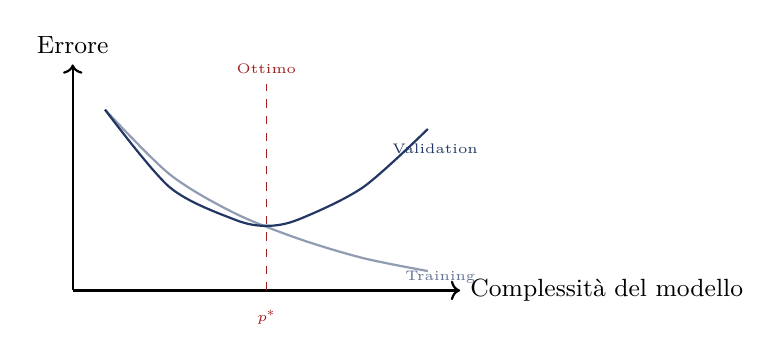
\begin{tikzpicture}[scale=0.82]
  \draw[thick,->] (0,0) -- (6,0) node[right,font=\small]{Complessità del modello};
  \draw[thick,->] (0,0) -- (0,3.5) node[above,font=\small]{Errore};
  % Training error
  \draw[thick,mblue!50] plot[smooth]
    coordinates {(0.5,2.8)(1.5,1.8)(2.5,1.2)(3.5,0.8)(4.5,0.5)(5.5,0.3)};
  \node[right,font=\tiny,mblue!70] at (5.0,0.2) {Training};
  % Validation error
  \draw[thick,mblue] plot[smooth]
    coordinates {(0.5,2.8)(1.5,1.6)(2.5,1.1)(3.0,1.0)(3.5,1.1)(4.5,1.6)(5.5,2.5)};
  \node[right,font=\tiny,mblue] at (4.8,2.2) {Validation};
  % Optimal
  \draw[dashed,mred] (3.0,0) -- (3.0,3.2)
    node[above,font=\tiny,mred]{Ottimo};
  \node[below,font=\tiny,mred] at (3.0,-0.15) {$p^*$};
\end{tikzpicture}
\end{center}
\end{frame}

\begin{frame}{Metodi di Selezione dei Predittori}
\phantomsection\label{metodi-di-selezione-dei-predittori}
\small

\textbf{Stepwise (forward, backward, entrambe)}

\begin{itemize}\footnotesize
\item \emph{Forward}: si parte da nessun predittore, si aggiunge uno alla volta il più significativo
\item \emph{Backward}: si parte da tutti, si rimuove il meno significativo
\item \emph{Stepwise}: combinazione forward + backward
\end{itemize}

\vspace{0.3em}

\textbf{Selezione basata su criteri di informazione}

\begin{itemize}\footnotesize
\item \textbf{AIC} (Akaike): penalizza per il numero di parametri; favorisce modelli predittivi
\item \textbf{BIC} (Bayesian): penalizza più severamente; tende a modelli più parsimoniosi
\end{itemize}

\vspace{0.3em}

\textbf{Selezione gerarchica (hierarchical / teorica)}

I predittori vengono aggiunti in blocchi teoricamente motivati, non
sulla base della significatività statistica.
\end{frame}

\begin{frame}{Problemi dei Metodi Stepwise}
\phantomsection\label{problemi-dei-metodi-stepwise}
\small

Lo stepwise automatico è \textbf{molto usato e molto criticato}:

\vspace{0.3em}

\begin{itemize}\small
\item \textbf{Inflazione del Type I error}: con molti predittori testati, la probabilità di trovare almeno un falso positivo esplode
\item \textbf{Instabilità}: piccole variazioni nei dati producono modelli finali molto diversi
\item \textbf{Sovrastima degli effect size}: i $\hat{\beta}$ dei predittori selezionati sono sistematicamente sovrastimati (\emph{winner's curse})
\item \textbf{Ignora la struttura teorica}: un predittore può essere escluso perché correlato ad altri, non perché irrilevante
\item \textbf{$p$-values non validi}: i $p$-value post-selezione non hanno la loro interpretazione nominale
\end{itemize}

\vspace{0.3em}

\footnotesize \textbf{Raccomandazione pratica}: preferire la selezione
\textbf{teorica/gerarchica} guidata da ipotesi e DAG. Se si usa
stepwise, validare il modello su un campione indipendente.

\vspace{0.2em}

\tiny Harrell (2015). \emph{Regression Modeling Strategies}. Springer.
Capitoli introduttivi Open Access: \url{https://hbiostat.org/rmsc/}
\end{frame}

\begin{frame}{Selezione Gerarchica (Hierarchical Regression)}
\phantomsection\label{selezione-gerarchica-hierarchical-regression}
\small

I predittori vengono inseriti in \textbf{blocchi} ordinati teoricamente,
e si valuta il contributo incrementale di ciascun blocco tramite il
cambiamento di \(R^2\) (o log-likelihood nella logistica).

\vspace{0.3em}

\textbf{Esempio neuropsicologico}:

\begin{center}
\begin{tabular}{clcc}
\toprule
\textbf{Blocco} & \textbf{Predittori} & $\boldsymbol{R^2}$ & $\boldsymbol{\Delta R^2}$ \\
\midrule
1 & Demografici (età, scolarità, sesso) & .18 & .18*** \\
2 & + Biomarkers imaging (volume ippocampale) & .29 & .11*** \\
3 & + Score neuropsicologici (MMSE, memoria) & .41 & .12*** \\
\bottomrule
\end{tabular}
\end{center}
\vspace{0.3em}

\small In questa logica, ogni blocco è inserito
\textbf{per ragioni teoriche}, non perché significativo. Il
\(\Delta R^2\) risponde alla domanda: ``I biomarkers aggiungono potere
esplicativo al di là dei soli dati demografici?''
\end{frame}

\section{Diagnostiche del Modello}\label{diagnostiche-del-modello}

\begin{frame}{Diagnostiche della Regressione Lineare}
\phantomsection\label{diagnostiche-della-regressione-lineare}
% [IMMAGINE SUGGERITA: i 4 plot diagnostici classici di R: Residuals vs Fitted,
%  Normal Q-Q, Scale-Location, Residuals vs Leverage]

\small

I \textbf{residui} (\(\hat{\varepsilon}_i = Y_i - \hat{Y}_i\)) devono
soddisfare le assunzioni del modello. I grafici diagnostici principali:

\vspace{0.3em}

\begin{columns}
\column{0.5\textwidth}
\begin{itemize}\footnotesize
\item \textbf{Residuals vs Fitted}: deve essere nuvola casuale (no pattern $\Rightarrow$ linearità OK, omoschedasticità OK)
\item \textbf{Normal Q-Q}: i residui devono seguire la diagonale (normalità dei residui)
\end{itemize}
\column{0.5\textwidth}
\begin{itemize}\footnotesize
\item \textbf{Scale-Location}: per verificare omoschedasticità (varianza costante)
\item \textbf{Cook's distance / Leverage}: individua i punti influenti (\emph{outliers} che distorcono la retta)
\end{itemize}
\end{columns}

\vspace{0.4em}

\small \textbf{In R}: \texttt{plot(modello)} produce automaticamente
questi 4 grafici. \texttt{car::vif(modello)} calcola il VIF per la
multicollinearità.
\end{frame}

\begin{frame}{Diagnostiche: Problemi Comuni}
\phantomsection\label{diagnostiche-problemi-comuni}
\small

\textbf{Multicollinearità}: due o più predittori sono altamente
correlati tra loro.

\begin{itemize}\footnotesize
\item Sintomo: SE grandi, coefficienti instabili, cambi di segno aggiungendo predittori
\item Diagnosi: VIF (Variance Inflation Factor) --- VIF $> 5$--$10$ indica problema
\item Soluzione: rimuovere uno dei predittori correlati, usare PCA, o centrare le variabili
\end{itemize}

\vspace{0.3em}

\textbf{Outliers e osservazioni influenti}:

\begin{itemize}\footnotesize
\item \emph{Outlier}: residuo molto grande (soggetto mal predetto)
\item \emph{Leverage}: osservazione con valore estremo nei predittori
\item \emph{Osservazione influente}: rimuovendola, il modello cambia sostanzialmente (Cook's $D > 1$)
\end{itemize}

\vspace{0.3em}

\textbf{Eteroschedasticità}: la varianza dei residui non è costante
(es.~aumenta con \(\hat{Y}\)). Soluzione: trasformazione di \(Y\)
(es.~log), o errori robusti (HC).

\vspace{0.3em}

\textbf{Specificazione del modello}: relazione non lineare tra \(X\) e
\(Y\) --- aggiungere termine quadratico o usare GAM.
\end{frame}

\begin{frame}{Diagnostiche della Regressione Logistica}
\phantomsection\label{diagnostiche-della-regressione-logistica}
\small

\textbf{Calibrazione}: il modello prevede probabilità accurate?

\begin{itemize}\footnotesize
\item \textbf{Hosmer-Lemeshow test}: divide i soggetti in decili di probabilità predetta e confronta frequenze osservate vs attese. $p > .05$ indica buona calibrazione.
\item \textbf{Calibration plot}: probabilità predetta (asse $x$) vs proporzione osservata (asse $y$) --- la curva deve stare vicina alla diagonale.
\end{itemize}

\vspace{0.3em}

\textbf{Discriminazione}: il modello distingue bene i casi dai non-casi?

\begin{itemize}\footnotesize
\item \textbf{AUC-ROC}: 0.5 = caso, 1.0 = perfetto. Valori $> 0.75$--$0.80$ sono considerati accettabili in clinica.
\item \textbf{Sensibilità e Specificità} al cut-off ottimale (es.\ Youden Index).
\end{itemize}

\vspace{0.3em}

\textbf{Separazione completa} (\emph{perfect separation}): se un
predittore separa perfettamente i due gruppi, il modello non converge.
Soluzione: regressione logistica penalizzata (Firth).
\end{frame}

\section{Il Problema dell'Inclusione dei
Predittori}\label{il-problema-dellinclusione-dei-predittori}

\begin{frame}{Non Tutti i Predittori Devono Essere Controllati}
\phantomsection\label{non-tutti-i-predittori-devono-essere-controllati}
\small

Un errore frequente nella pratica: inserire nel modello
\textbf{tutte le variabili disponibili} o tutte quelle correlate con
l'outcome, senza ragionare sulla struttura causale.

\vspace{0.4em}

Come discusso nella \textbf{Sezione 3 (DAG)}, il tipo di variabile che
si inserisce nel modello cambia il significato del coefficiente stimato:
\vspace{0.3em}

\begin{center}
\begin{tabular}{>{\footnotesize}l >{\footnotesize}l >{\footnotesize}p{4.8cm}}
\toprule
\textbf{Struttura} & \textbf{Controllare?} & \textbf{Conseguenza se si controlla} \\
\midrule
Confounder & \textbf{Sì} & Rimuove associazione spuria tra $X$ e $Y$ \\
Mediatore  & \textbf{Dipende} & Blocca parte dell'effetto causale di $X$ su $Y$ \\
Collider   & \textbf{No} & Introduce un'associazione spuria (bias di selezione) \\
Variabile irrilevante & \textbf{No} & Riduce potere statistico e aumenta SE \\
\bottomrule
\end{tabular}
\end{center}

\vspace{0.2em}

\small \(\Rightarrow\)
\textbf{La costruzione del modello deve partire da un DAG, non dai $p$-value.}\textbackslash{}
\small \(\Rightarrow\) Per approfondimento: \textbf{Sezione 3}, slide su
DAG, confounders e colliders.
\end{frame}

\begin{frame}{Il Collider nella Regressione: Un Esempio}
\phantomsection\label{il-collider-nella-regressione-un-esempio}
\begin{center}
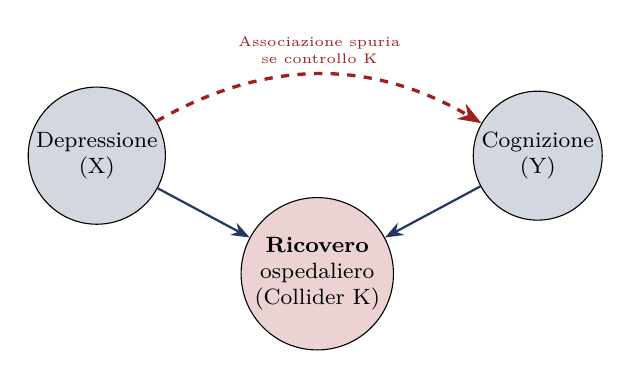
\begin{tikzpicture}[
  node/.style={circle,draw,fill=mblue!20,font=\footnotesize,
               minimum size=1.1cm,inner sep=1pt,align=center},
  coll/.style={circle,draw,fill=mred!20,font=\footnotesize,
               minimum size=1.1cm,inner sep=1pt,align=center},
  arr/.style={-{Stealth},mblue,thick},
  spurious/.style={-{Stealth},mred,dashed,very thick}
]
\node[node, align=center] (dep)  at (-2.8,2)  {Depressione\\(X)};
\node[node, align=center] (cog)  at ( 2.8,2)  {Cognizione\\(Y)};
\node[coll, align=center] (osp)  at (0,0.5)   {\textbf{Ricovero}\\ospedaliero\\(Collider K)};

\draw[arr] (dep)--(osp);
\draw[arr] (cog)--(osp);
\draw[spurious] (dep) to[bend left=30]
  node[above,font=\tiny,mred, align=center]{Associazione spuria\\se controllo K} (cog);
\end{tikzpicture}
\end{center}
\vspace{-0.3em}

\small Depressione e cognizione sono indipendenti nella popolazione
generale. Ma entrambe predicono il ricovero. Se analizziamo
\textbf{solo pazienti ricoverati} (o controlliamo per il ricovero),
troviamo una correlazione \emph{negativa} artificiosa tra depressione e
cognizione.

\vspace{0.2em}

\footnotesize Questo è il \textbf{Berkson's bias} --- frequente negli
studi condotti su campioni clinici.\textbackslash{} \(\Rightarrow\)
\textbf{Sezione 3} per approfondimento.
\end{frame}

\begin{frame}{La Regola dei 10 (e 20) Eventi per Predittore}
\phantomsection\label{la-regola-dei-10-e-20-eventi-per-predittore}
\small

Nella regressione logistica, il numero di predittori che si possono
stimare in modo affidabile dipende dal numero di \textbf{eventi}
(categoria meno frequente), non dal numero totale di soggetti.

\vspace{0.3em}

\textbf{Regola empirica classica}: almeno \textbf{10 eventi per
predittore} (EPV = Events Per Variable).

\vspace{0.3em}

\textbf{Ricerca recente}: la regola dei 10 EPV può non essere
sufficiente; si raccomanda spesso 20 EPV o l'uso di metodi di shrinkage
(Ridge, LASSO).

\vspace{0.4em}

\textbf{Esempio pratico}:

\begin{itemize}\footnotesize
\item $N = 200$ soggetti MCI, 40 convertono ad AD (EPV = 40)
\item Con EPV = 40 si possono stimare in modo affidabile fino a $\sim$4 predittori (regola dei 10)
\item Inserirne 8 causerebbe overfitting anche con $N = 200$
\end{itemize}

\vspace{0.2em}

\tiny Riley et al.~(2019). Minimum sample size for developing a
multivariable prediction model. \emph{Stat Med}. Open Access:
\url{https://doi.org/10.1002/sim.7993}
\end{frame}

\begin{frame}
\end{frame}

\section{Riepilogo}\label{riepilogo}

\begin{frame}{Riepilogo: Lineare vs Logistica}
\phantomsection\label{riepilogo-lineare-vs-logistica}
\begin{center}
\begin{tabular}{>{\small}l >{\small}l >{\small}l}
\toprule
 & \textbf{Regressione Lineare} & \textbf{Regressione Logistica} \\
\midrule
Outcome    & Continuo ($Y \in \mathbb{R}$) & Binario ($Y \in \{0,1\}$) \\
Stima      & Minimi quadrati (OLS) & Massima verosimiglianza \\
Coefficiente & $\hat{\beta}$: variazione di $Y$ & $\hat{\beta}$: variazione log-odds \\
Effetto    & $\hat{\beta}$ directo & OR = $e^{\hat{\beta}}$ \\
Fit        & $R^2$, RMSE & AUC, pseudo-$R^2$, HL \\
Diagnostica & Residui, Q-Q, Cook's $D$ & Calibrazione, separazione \\
\bottomrule
\end{tabular}
\end{center}
\vspace{0.5em}
\small \textbf{Regola d'oro comune a entrambi}: costruire il modello sulla base di ipotesi teoriche e DAG, non sulla base di stepwise automatico o significatività statistica.
\end{frame}

\begin{frame}{Risorse Open Access}
\phantomsection\label{risorse-open-access}
\small

\begin{itemize}\footnotesize

\item \textbf{Harrell (2015). Regression Modeling Strategies}. Materiali online:\\
  \url{https://hbiostat.org/rmsc/}

\item \textbf{Riley et al.\ (2019). Sample size for prediction models}. \emph{Stat Med}.\\
  \url{https://doi.org/10.1002/sim.7993}

\item \textbf{OR vs RR}: Cummings (2009). \emph{Am J Epidemiol} 171(6).\\
  \url{https://doi.org/10.1093/aje/kwp440}

\item \textbf{LASSO e Ridge}: Tibshirani (1996). \emph{J R Stat Soc B}. (Fondamentale per shrinkage)\\
  \url{https://doi.org/10.1111/j.2517-6161.1996.tb02080.x}

\item \textbf{Pacchetto R \texttt{rms}} (Harrell): regressione avanzata, calibrazione, validazione.\\
  \url{https://cran.r-project.org/package=rms}

\item \textbf{DAGitty}: per costruire DAG prima di scegliere i predittori.\\
  \url{https://www.dagitty.net}

\item \textbf{Sievert (2020). Interactive Web-Based Data Visualization with R} (plotly, ggplot2).\\
  Libro Open Access: \url{https://plotly-r.com}

\item \textbf{The Effect Book (Huntington-Klein)}: cap.\ su OLS e regressione logistica.\\
  \url{https://theeffectbook.net}

\end{itemize}
\end{frame}




\end{document}
